% Options for packages loaded elsewhere
% Options for packages loaded elsewhere
\PassOptionsToPackage{unicode}{hyperref}
\PassOptionsToPackage{hyphens}{url}
\PassOptionsToPackage{dvipsnames,svgnames,x11names}{xcolor}
%
\documentclass[
]{article}
\usepackage{xcolor}
\usepackage[margin=2.5cm]{geometry}
\usepackage{amsmath,amssymb}
\setcounter{secnumdepth}{5}
\usepackage{iftex}
\ifPDFTeX
  \usepackage[T1]{fontenc}
  \usepackage[utf8]{inputenc}
  \usepackage{textcomp} % provide euro and other symbols
\else % if luatex or xetex
  \usepackage{unicode-math} % this also loads fontspec
  \defaultfontfeatures{Scale=MatchLowercase}
  \defaultfontfeatures[\rmfamily]{Ligatures=TeX,Scale=1}
\fi
\usepackage{lmodern}
\ifPDFTeX\else
  % xetex/luatex font selection
\fi
% Use upquote if available, for straight quotes in verbatim environments
\IfFileExists{upquote.sty}{\usepackage{upquote}}{}
\IfFileExists{microtype.sty}{% use microtype if available
  \usepackage[]{microtype}
  \UseMicrotypeSet[protrusion]{basicmath} % disable protrusion for tt fonts
}{}
\makeatletter
\@ifundefined{KOMAClassName}{% if non-KOMA class
  \IfFileExists{parskip.sty}{%
    \usepackage{parskip}
  }{% else
    \setlength{\parindent}{0pt}
    \setlength{\parskip}{6pt plus 2pt minus 1pt}}
}{% if KOMA class
  \KOMAoptions{parskip=half}}
\makeatother
% Make \paragraph and \subparagraph free-standing
\makeatletter
\ifx\paragraph\undefined\else
  \let\oldparagraph\paragraph
  \renewcommand{\paragraph}{
    \@ifstar
      \xxxParagraphStar
      \xxxParagraphNoStar
  }
  \newcommand{\xxxParagraphStar}[1]{\oldparagraph*{#1}\mbox{}}
  \newcommand{\xxxParagraphNoStar}[1]{\oldparagraph{#1}\mbox{}}
\fi
\ifx\subparagraph\undefined\else
  \let\oldsubparagraph\subparagraph
  \renewcommand{\subparagraph}{
    \@ifstar
      \xxxSubParagraphStar
      \xxxSubParagraphNoStar
  }
  \newcommand{\xxxSubParagraphStar}[1]{\oldsubparagraph*{#1}\mbox{}}
  \newcommand{\xxxSubParagraphNoStar}[1]{\oldsubparagraph{#1}\mbox{}}
\fi
\makeatother


\usepackage{longtable,booktabs,array}
\usepackage{calc} % for calculating minipage widths
% Correct order of tables after \paragraph or \subparagraph
\usepackage{etoolbox}
\makeatletter
\patchcmd\longtable{\par}{\if@noskipsec\mbox{}\fi\par}{}{}
\makeatother
% Allow footnotes in longtable head/foot
\IfFileExists{footnotehyper.sty}{\usepackage{footnotehyper}}{\usepackage{footnote}}
\makesavenoteenv{longtable}
\usepackage{graphicx}
\makeatletter
\newsavebox\pandoc@box
\newcommand*\pandocbounded[1]{% scales image to fit in text height/width
  \sbox\pandoc@box{#1}%
  \Gscale@div\@tempa{\textheight}{\dimexpr\ht\pandoc@box+\dp\pandoc@box\relax}%
  \Gscale@div\@tempb{\linewidth}{\wd\pandoc@box}%
  \ifdim\@tempb\p@<\@tempa\p@\let\@tempa\@tempb\fi% select the smaller of both
  \ifdim\@tempa\p@<\p@\scalebox{\@tempa}{\usebox\pandoc@box}%
  \else\usebox{\pandoc@box}%
  \fi%
}
% Set default figure placement to htbp
\def\fps@figure{htbp}
\makeatother


% definitions for citeproc citations
\NewDocumentCommand\citeproctext{}{}
\NewDocumentCommand\citeproc{mm}{%
  \begingroup\def\citeproctext{#2}\cite{#1}\endgroup}
\makeatletter
 % allow citations to break across lines
 \let\@cite@ofmt\@firstofone
 % avoid brackets around text for \cite:
 \def\@biblabel#1{}
 \def\@cite#1#2{{#1\if@tempswa , #2\fi}}
\makeatother
\newlength{\cslhangindent}
\setlength{\cslhangindent}{1.5em}
\newlength{\csllabelwidth}
\setlength{\csllabelwidth}{3em}
\newenvironment{CSLReferences}[2] % #1 hanging-indent, #2 entry-spacing
 {\begin{list}{}{%
  \setlength{\itemindent}{0pt}
  \setlength{\leftmargin}{0pt}
  \setlength{\parsep}{0pt}
  % turn on hanging indent if param 1 is 1
  \ifodd #1
   \setlength{\leftmargin}{\cslhangindent}
   \setlength{\itemindent}{-1\cslhangindent}
  \fi
  % set entry spacing
  \setlength{\itemsep}{#2\baselineskip}}}
 {\end{list}}
\usepackage{calc}
\newcommand{\CSLBlock}[1]{\hfill\break\parbox[t]{\linewidth}{\strut\ignorespaces#1\strut}}
\newcommand{\CSLLeftMargin}[1]{\parbox[t]{\csllabelwidth}{\strut#1\strut}}
\newcommand{\CSLRightInline}[1]{\parbox[t]{\linewidth - \csllabelwidth}{\strut#1\strut}}
\newcommand{\CSLIndent}[1]{\hspace{\cslhangindent}#1}



\setlength{\emergencystretch}{3em} % prevent overfull lines

\providecommand{\tightlist}{%
  \setlength{\itemsep}{0pt}\setlength{\parskip}{0pt}}



 


\makeatletter
\@ifpackageloaded{caption}{}{\usepackage{caption}}
\AtBeginDocument{%
\ifdefined\contentsname
  \renewcommand*\contentsname{Table of contents}
\else
  \newcommand\contentsname{Table of contents}
\fi
\ifdefined\listfigurename
  \renewcommand*\listfigurename{List of Figures}
\else
  \newcommand\listfigurename{List of Figures}
\fi
\ifdefined\listtablename
  \renewcommand*\listtablename{List of Tables}
\else
  \newcommand\listtablename{List of Tables}
\fi
\ifdefined\figurename
  \renewcommand*\figurename{Figure}
\else
  \newcommand\figurename{Figure}
\fi
\ifdefined\tablename
  \renewcommand*\tablename{Table}
\else
  \newcommand\tablename{Table}
\fi
}
\@ifpackageloaded{float}{}{\usepackage{float}}
\floatstyle{ruled}
\@ifundefined{c@chapter}{\newfloat{codelisting}{h}{lop}}{\newfloat{codelisting}{h}{lop}[chapter]}
\floatname{codelisting}{Listing}
\newcommand*\listoflistings{\listof{codelisting}{List of Listings}}
\makeatother
\makeatletter
\makeatother
\makeatletter
\@ifpackageloaded{caption}{}{\usepackage{caption}}
\@ifpackageloaded{subcaption}{}{\usepackage{subcaption}}
\makeatother
\usepackage{bookmark}
\IfFileExists{xurl.sty}{\usepackage{xurl}}{} % add URL line breaks if available
\urlstyle{same}
\hypersetup{
  pdftitle={Modeling drifter trajectories and ensemble dispersion from the Ocean Training Course 2025},
  colorlinks=true,
  linkcolor={blue},
  filecolor={Maroon},
  citecolor={Blue},
  urlcolor={Blue},
  pdfcreator={LaTeX via pandoc}}


\title{\textbf{Modeling drifter trajectories and ensemble dispersion
from the Ocean Training Course 2025}}
\author{Samantha Kucher \and Vadim Bertrand}
\date{}
\begin{document}
\maketitle

\renewcommand*\contentsname{Table of contents}
{
\hypersetup{linkcolor=}
\setcounter{tocdepth}{3}
\tableofcontents
}

\newpage{}

\section{Introduction}\label{introduction}

Better understanding of particle transport in the ocean is crucial to
reduce marine plastic pollution. The life of microplastics in the ocean
is nonetheless complex: they can be transported through long distances
by currents and gyres, mixed in turbulent flows, broken into smaller
pieces, and sinked by biofouling
(\citeproc{ref-sutherland2023fluid}{Sutherland et al., 2023}). Recent
laboratory experiments and theoretical developments have been made to
study the influence of particle size, shape and density
(\citeproc{ref-clark2020settling}{Clark et al., 2020}),
(\citeproc{ref-dibenedetto2022enhanced}{DiBenedetto et al., 2022}),
(\citeproc{ref-calvert2024laboratory}{R. Calvert et al., 2024}). There
is a growing interest in narrowing the gap between controlled
experiments and real-world conditions found in the ocean.

Oceanic models are able to forecast the ocean state several days ahead,
but they are not capable of resolving the small scales corresponding to
particle transport. The combined effect of waves, currents and wind must
be taken into account to predict the drift of passive tracers
(\citeproc{ref-christensen2018short}{Christensen et al., 2018}).
Parametrizing the movement of particles in wavy, turbulent flows thus
presents a fundamental challenge (\citeproc{ref-van2020physical}{Van
Sebille et al., 2020}), (\citeproc{ref-sutherland2023fluid}{Sutherland
et al., 2023}).

It has been shown that large non-Lagrangian floating particles
experience a drift larger than the Stokes drift
(\citeproc{ref-calvert2021mechanism}{Ross Calvert et al., 2021}). This
is due to the object oscillation relative to the free surface and its
submergence, which changes continuously with the wave slope. The size of
the object with respect to the wavelength is a determining factor in the
drifting velocity. In the ocean, the dynamics of currents strongly
impacts the propagation of wave fields
(\citeproc{ref-quilfen2019ocean}{Quilfen \& Chapron, 2019}), and
therefore modifies the particles trajectories. The impact of wind has
also been addressed, using a leeway modeling approach to gain physical
understanding of the forces that play a role in the drift of floating
objects (\citeproc{ref-wagner2022winds}{Wagner et al., 2022}). This
model, however, does not accurately predict the trajectories of floating
particles. Such prediction is given by the Maxey-Riley set for inertial
surface particles Beron-Vera et al.
(\citeproc{ref-beron2019building}{2019}).

Satellite-tracked drifters have been studied in the North Atlantic
(\citeproc{ref-elipot2016global}{S. Elipot et al., 2016}), and an
\emph{in-situ} study has been made in the Florida Current
(\citeproc{ref-olascoaga2020observation}{Olascoaga et al., 2020}). In
the latter, the trajectory of buoys has been followed for one week. The
authors successfully modeled the experimental data using a framework
derived from the Maxey-Riley equations.

This project aims to reconstruct the trajectory of drifters deployed
during the expedition and to better understand how physical processes
govern their motion. We thus need to take into account the satellite
measurements of sea surface deformation, wave induced currents and wind
speed. We employ a two folded approach: (i) in first approximation a
linear combination of the surface currents, Stokes drift and direct
wind-force, and (ii) the full equations describing the dynamics of
floating intertial particles in the ocean: the Maxey-Riley set. These
two methods will allow us to decompose and analyze the individual forces
governing the drifter's motion, providing deeper insights into the
underlying dynamics.

We focus here on deterministic modellings of the drift. However, given
the inherent chaotic nature of the problem and the uncertainties carried
by our observations of oceanic and atmospheric variables, stochastic
approaches might be relevant to simulate ensemble of probable and
realistic trajectories, rather than one \emph{incorrect} estimate. One
challenge is to control the dispersion of simulated ensembles to
accurately cover the distribution of possible trajectories. To address
this question we study the relative dispersion over time of several
ensembles of drifters deployed at the same space-time position.

\section{Instruments, data and
methods}\label{instruments-data-and-methods}

This section describes the two types of drifters deployed during OTC25,
as well as the data and trajectory reconstruction methods used in our
analysis. We first present the design of the MELODI and SPOT drifters.
Next, we introduce the different satellite-derived and drifter datasets
(including the preprocessing steps applied when relevant). Finally, we
detail the Lagrangian statistics used to characterize the drift
dynamics, the trajectory reconstruction methods implemented, and the
metrics employed to evaluate them.

\subsection{Drifters deployed during the
campaign}\label{drifters-deployed-during-the-campaign}

Figure~\ref{fig-drifters} shows a photograph of all drifter types
deployed during the campaign, with the exception of the Sofar Spotter.
At the time of writing, only eOdyn MELODI and IGE SPOT data are
available, and we therefore focus on these two types. However, it should
be noted that 16 OpenMetBuoy, 4 CLS MARGE-T II, and 1 Sofar Spotter buoy
were also deployed. Including these additional drifters would strengthen
our analysis, as we will discuss in Section~\ref{sec-disc}.

\begin{figure}

\centering{

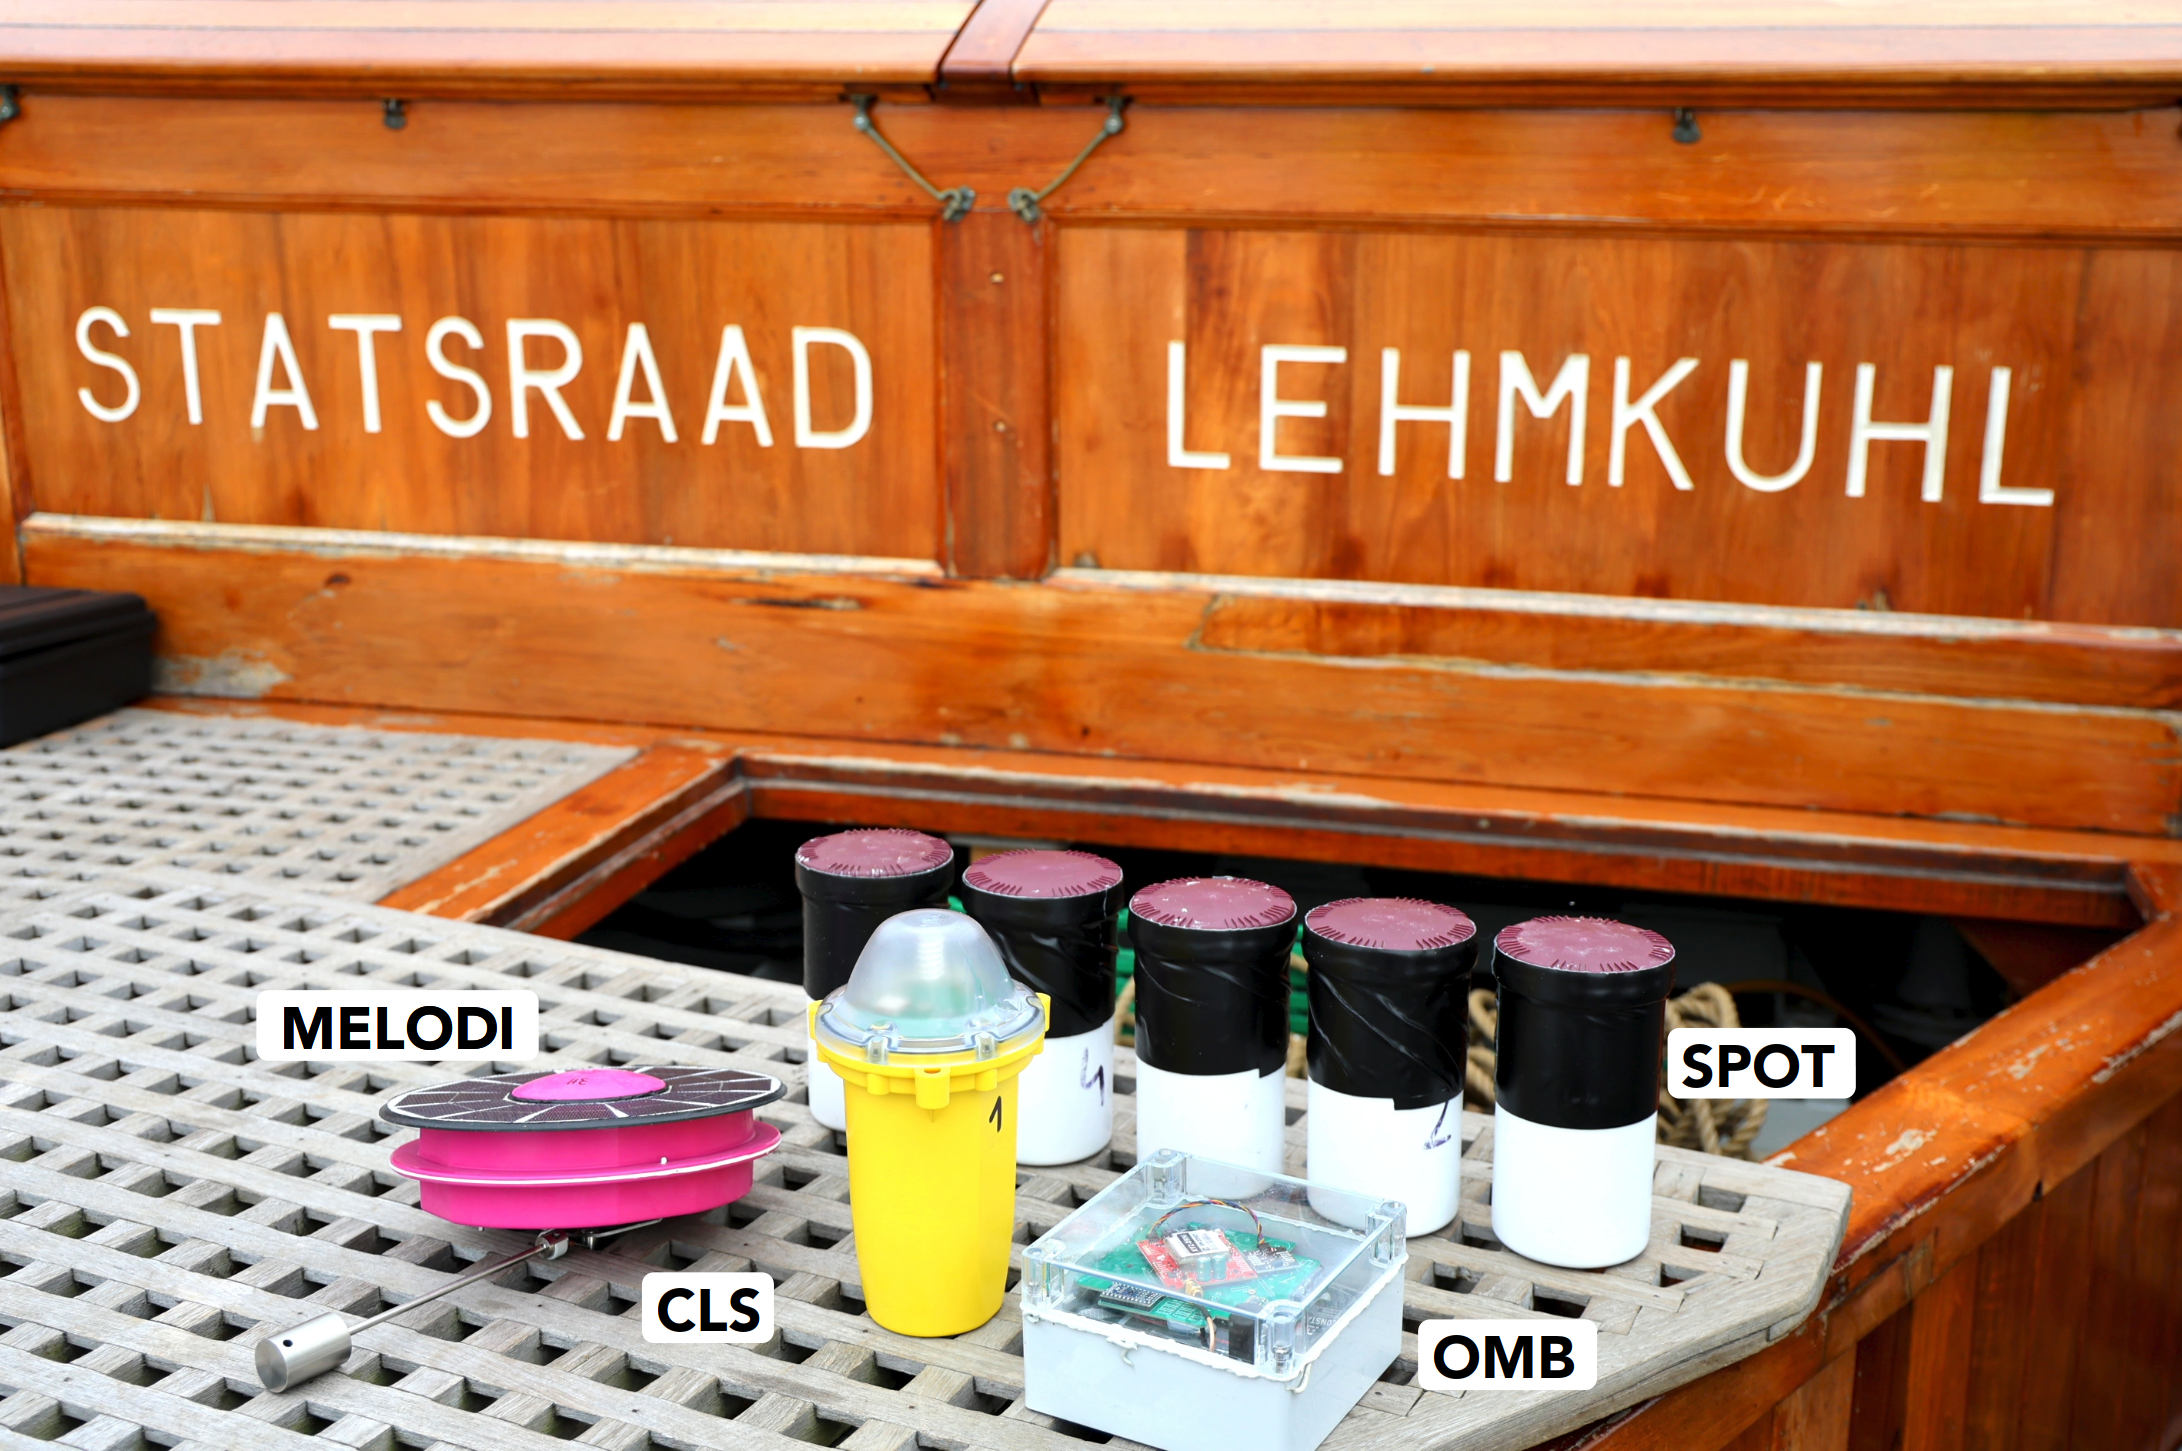
\includegraphics[width=0.7\linewidth,height=\textheight,keepaspectratio]{images/drifters.png}

}

\caption{\label{fig-drifters}Types of drifters deployed during the OTC25
campaign between Tromsø and Nice. There was also a Sofar drifter not
shown in the picture. Photo taken by Joël Marc.}

\end{figure}%

\subsubsection{MELODI}\label{melodi}

The MELODI (\citeproc{ref-MELODI}{{``MELODI,''} 2024}) is a surface
drifter developed by the company eOdyn. Although we are only interested
in the drifter's position, it also measures surface currents, surface
temperature and wave parameters. The position is determined using
several satellite constellations, with a sampling frequency of 1 hour.
The drifter uses the Iridium satellite network to transmit its data. It
is powered by four Li-ion 3500 mAh, 3.7 V batteries and a 6 W solar
panel, which allows it to operate for at least several months. Thanks to
its low-profile, see Figure~\ref{fig-melodi-design}, the MELODI drifter
is expected to be only weakly affected by wind drift.

\begin{figure}

\centering{

\includegraphics[width=0.5\linewidth,height=\textheight,keepaspectratio]{images/melodi-design.png}

}

\caption{\label{fig-melodi-design}Design of the MELODI drifter}

\end{figure}%

From Tromsø to Nice, 18 MELODI drifters were deployed in various
locations: in the North Sea and its Lofoten eddy, in the North Atlantic
(including during a storm event), before and after the Strait of
Gibraltar (within the Alboran eddy), and in the western Mediterranean
Sea. This can be seen in Figure~\ref{fig-drifter-deployments}.

\begin{figure}[H]

\centering{

\pandocbounded{\includegraphics[keepaspectratio]{index_files/figure-latex/sections-02_methods-fig-drifter-deployments-output-1.png}}

}

\caption{\label{fig-drifter-deployments}MELODI and SPOT drifter
deployments during the OTC25 campaign.}

\end{figure}%

\subsubsection{SPOT}\label{spot}

The SPOT (\citeproc{ref-SPOT}{{``SPOT,''} 2024}) is a home-made surface
drifter designed and developed at Institut des Géosciences de
l'Environnement (IGE). Its design is very simple, see
Figure~\ref{fig-spot-design}: a weighted waterproof jar containing a GPS
tracer powered by external batteries. The GPS tracer is a SPOT Trace,
which uses the Globalstar satellite network to transmit its position
every 30 minutes. External batteries (4 LR20 alkaline 1.5V 13Ah) allow
the drifter to operate for up to 6 months and counting at the time of
writing.

\begin{figure}

\centering{

\includegraphics[width=0.75\linewidth,height=\textheight,keepaspectratio]{images/spot-design.png}

}

\caption{\label{fig-spot-design}Design of the SPOT drifter}

\end{figure}%

During the first deployments we noticed that the SPOT drifters exhibited
an orbital motion around their vertical axis and we suspected that it
was the cause for the observed effective sampling frequency being larger
than the nominal 30 minutes (see
Figure~\ref{fig-spot-sampling-frequency}). To mitigate this motion we
designed a dynamic anchor attached to the bottom of the drifter. Being
at sea we had to reuse material available aboard the ship: old sails and
steel wire ropes, as visible in Figure~\ref{fig-spot-anchor}.

\begin{figure}

\centering{

\includegraphics[width=0.7\linewidth,height=\textheight,keepaspectratio]{images/IMG_0538.jpeg}

}

\caption{\label{fig-spot-anchor}SPOT drifter with a dynamic anchor}

\end{figure}%

The last five drifters deployed in the Mediterranean Sea were equipped
with this anchor. Using the drifter data presented in
Section~\ref{sec-data-drif-traj} it seems that the anchor was effective
in improving the effective sampling frequency, as shown in the left
panel of Figure~\ref{fig-spot-sampling-frequency}. However, the right
panel of Figure~\ref{fig-spot-sampling-frequency} indicates that, among
the drifters deployed in the Mediterranean Sea, drifter \#19 stopped
emitting very shortly after deployment for an unknown reason, while
drifters \#16 and \#18 beached soon after deployment, leaving only
drifters \#17 and \#20 active for more than a month. In addition, the
Mediterranean Sea is known for its quieter sea state compared to the
North Atlantic and the Bay of Biscay, which could explain the improved
effective sampling resolution. Further analysis is therefore required to
confirm whether the drogue was indeed effective.

\begin{figure}[H]

\centering{

\pandocbounded{\includegraphics[keepaspectratio]{index_files/figure-latex/sections-02_methods-fig-spot-sampling-frequency-output-1.png}}

}

\caption{\label{fig-spot-sampling-frequency}SPOT drifters effective
sampling period. The dashed blue line indicates the nominal sampling
period of 30 minutes.}

\end{figure}%

\subsection{Satellite and drifter
data}\label{satellite-and-drifter-data}

Our analysis requires both maps of geophysical quantities (surface
currents, waves, winds) and lagrangian drifter trajectories.

\subsubsection{Satellite-derived gridded
products}\label{sec-data-gridded-products}

Geophysical quantities of interest are derived from satellite
observations, assimilated in physical models of varying complexity.

\paragraph{Sea Surface Height}\label{sea-surface-height}

VarDyn is a variational mapping method jointly reconstructing Sea
Surface Height (SSH) and Sea Surface Temperature (SST)
(\citeproc{ref-leguillouVarDynDynamicalJointReconstructions2025}{Le
Guillou et al., 2025}). The version used in our analysis assimilates
both SWOT KaRin and Nadir altimeters data and produces daily 0.05°
\(\times\) 0.05° maps. This dataset provides both SSH and sea surface
currents, derived from the SSH field.

\paragraph{Sea Surface Wind}\label{sea-surface-wind}

Wind acts both directly on the drifter (the leeway) and indirectly
through its effect on waves and currents. We use the wind velocity and
stress at the surface from the 0.125° \(\times\) 0.125° hourly ECMWF
bias corrected product
(\citeproc{ref-SeaSurfaceWind}{WIND\_GLO\_PHY\_L4\_NRT\_012\_004, 2024})
developed by the Royal Netherlands Meteorological Institute.

\paragraph{Sea State}\label{sea-state}

Waves also affect drifter trajectories through the Stokes drift. We
employ the Stokes drift obtained by assimilating significant wave height
in the wave model MFWAM, available in the 0.083° \(\times\) 0.083°
hourly Global Ocean Waves Analysis and Forecast product
(\citeproc{ref-SeaState}{GLOBAL\_ANALYSISFORECAST\_WAV\_001\_027, 2023})
developed by Mercator Ocean International.

\subsubsection{Drifter data}\label{sec-data-drif-traj}

Starting from the raw GPS positions transmitted by the drifters, we
perform several preprocessing steps before using them in our analysis.

\paragraph{L0 version}\label{l0-version}

The L0 version of the data consists of datasets containing the original
timestamps and positions (latitude and longitude) for each drifter,
complemented by its deployment date and time. Each record also includes
the time interval between successive measurements.

\paragraph{L1 version}\label{l1-version}

The L1 version of the data is produced by applying the following Quality
Control (QC) steps to the L0 dataset:

\begin{enumerate}
\def\labelenumi{\arabic{enumi}.}
\tightlist
\item
  Spurious GPS locations were removed following the procedure described
  by Shane Elipot et al.
  (\citeproc{ref-elipotGlobalSurfaceDrifter2016}{2016}),
\item
  Curated trajectories were divided into segments whenever the time gap
  between two consecutive timestamps exceeded 6 hours,
\item
  Segments shorter than 1 day are discarded.
\end{enumerate}

As shown in Table~\ref{tbl-qc-numbers}, these QC steps result in only a
small reduction in the number of MELODI drifter observations. In
contrast, about 20\% of the SPOT observations were discarded, primarily
due to transmission issues that caused large gaps in the original
trajectories and consequently led to many short segments being removed.

\begin{longtable}[]{@{}lllll@{}}

\caption{\label{tbl-qc-numbers}Number of observations and segments in L0
and L1 versions for SPOT and MELODI datasets.}

\tabularnewline

\toprule\noalign{}
Dataset & \multicolumn{2}{l}{%
\# Observations} & \multicolumn{2}{l@{}}{%
\# Segments} \\
& L0 & L1 & L0 & L1 \\
\midrule\noalign{}
\endhead
\bottomrule\noalign{}
\endlastfoot
SPOT & 24503 & 19846 & 20 & 189 \\
MELODI & 47399 & 46837 & 19 & 39 \\

\end{longtable}

\paragraph{L2 version}\label{l2-version}

Trajectories are resampled at a regular time interval of 1 hour using a
linear interpolation for the positions and the velocities are then
computed using central differences.

An example of L0, L1 and L2 trajectories for a SPOT drifter is shown in
Figure~\ref{fig-drifter-processing}. It can be seen that the L0
trajectory contains some spurious points, which are removed in the L1
and L2 versions. Holes in the L1 and L2 trajectories correspond to gaps
larger than 6 hours in the original data. Holes are not filled by
interpolation in the L2 version as those trajectories are then
considered as distinct segments.

\begin{figure}[H]

\centering{

\pandocbounded{\includegraphics[keepaspectratio]{index_files/figure-latex/sections-02_methods-fig-drifter-processing-output-1.png}}

}

\caption{\label{fig-drifter-processing}SPOT drifter 0-4498291 data
(2025-05-12 -- 2025-09-16) at different pre-processing levels.}

\end{figure}%

Figure~\ref{fig-drifter-traj} presents the L2 trajectories of both SPOT
and MELODI drifters deployed between Tromsø and Nice during OTC25.

\begin{figure}[H]

\centering{

\pandocbounded{\includegraphics[keepaspectratio]{index_files/figure-latex/sections-02_methods-fig-drifter-traj-output-1.png}}

}

\caption{\label{fig-drifter-traj}L2 drifters data from the OTC 25
(2025-04-25 -- 2025-09-16).}

\end{figure}%

\subsection{Modeling of drifter trajectories}\label{sec-model-drif-traj}

This section describes the methods used to analyze the drifter
trajectories and reconstruct their positions. We first introduce the
trajectory reconstruction methods implemented in our analysis and we
detail the metrics employed to evaluate them. Next, we present the
Lagrangian statistics used to characterize the drift dynamics.

\subsubsection{Linear combination}\label{sec-linear-combination}

First, the drift is modeled as a simple linear combination of
geophysical forcings acting on the object:

\begin{equation}\phantomsection\label{eq-lin-comb-ode}{
\frac{d\mathbf{X}(t)}{dt} = (\mathbf{u}_{cg} + \mathbf{u}_e + \mathbf{u}_s + \beta_w \mathbf{u}_w)(t, \mathbf{X}(t))
}\end{equation}

where \(\mathbf{X}(t)\) is the position of the particle at time \(t\),
\(\mathbf{u}_{cg}\) is the current velocity vector field estimated from
\emph{balanced} SSH, \(\mathbf{u}_e\) is the wind-induced Ekman current
velocity vector field, \(\mathbf{u}_s\) is the wave-induced Stokes drift
velocity vector field, \(\mathbf{u}_w\) is the wind velocity vector
field at the sea surface, weighted by \(\beta_w\). The notation
\(( \cdot )(t, \mathbf{X}(t))\) indicates that the linear combination of
the velocity vector fields is interpolated in space and time at the
particle position.

The geostrophic approximation is the method classically employed in
operational products to derive sea surface currents from SSH by solving
the equilibrium between the Coriolis (pseudo-)force and the pressure
gradient: \begin{equation}\phantomsection\label{eq-geos-balance}{
f \mathbf{k} \times \mathbf{u}_g = -g \nabla \eta
}\end{equation} where \(f\) is the Coriolis parameter, \(\mathbf{k}\) is
the vertical unit vector, \(\mathbf{u}_g\) the geostrophic velocity
vector, \(g\) is the gravitational acceleration and \(\eta\) is the SSH.
The geostrophic balance neglects, in particular, the centrifugial
acceleration of the flow. This advective term can become significant in
intense mesoscale eddies, rings and meanders
(\citeproc{ref-penvenCyclogeostrophicBalanceMozambique2014}{Penven et
al., 2014}) or in submesoscale structures
(\citeproc{ref-archerWideswathSatelliteAltimetry2025}{Archer et al.,
2025}; \citeproc{ref-tranchantSWOTRevealsFineScale2025}{Tranchant et
al., 2025}). Accounting for the advection of momentum leads to the
cyclogeostrophic equilibrium:
\begin{equation}\phantomsection\label{eq-cyclogeos-balance}{
\mathbf{u}_{cg} - \frac{\mathbf{k}}{f} \wedge (\mathbf{u}_{cg} \cdot \nabla)\mathbf{u}_{cg} =  \mathbf{u}_g
}\end{equation} where \(\mathbf{u}_{cg}\) is the cyclogeostrophic
velocity vector. Solving the cyclogoeostrophic equation cannot be done
analyticaly in the general case
(\citeproc{ref-penvenCyclogeostrophicBalanceMozambique2014}{Penven et
al., 2014}); therefore the VarDyn product uses the cyclogeostrophic
inversion method proposed by Bertrand, Le Sommer, et al.
(\citeproc{ref-bertrandRobustVariationalFramework2025}{2025}) and
implemented in the Python package \texttt{jaxparrow}
(\citeproc{ref-bertrandJaxparrow2025}{Bertrand, Vianna Zaia De Almeida,
et al., 2025}).

Following classical Ekman theory (\citeproc{ref-ekman1905}{Ekman,
1905}), we estimate the Ekman currents at the sea surface as a function
of the wind stress at the sea surface provided by ECMWF:
\begin{equation}\phantomsection\label{eq-ekman-surface}{
\mathbf{u}_e = \frac{1}{\rho \sqrt{2 A_z |f|}} \tau e^{i \theta_e}
}\end{equation} where \(\theta_e = 45 °\) controls the deflection of the
wind stress vector \(\tau\) (should be multiplied by -1 in the North
Emisphere), \(\rho\) is the seawater density, and \(A_z\) is the
vertical eddy viscosity.

The Stokes drift and the wind velocity at the sea surface are directly
taken from the observation products as detailed in
Section~\ref{sec-data-gridded-products}.

\paragraph{Parameters estimation}\label{sec-lin-comb-param-estimation}

Our linear combination model has two free parameters that we propose to
tune from the drifters data. The vertical eddy viscosity \(A_z\) is
linked to the Ekman depth and varies depending on the mixing conditions
in the upper ocean. It is expected to range from
\(10^{-2} \text{ m}^2\text{s}^{-1}\) to
\(10^{-1}\text{ m}^2 \text{s}^{-1}\) in the open ocean under moderate
mixing. As the geometry of the drifter does not enter into consideration
here, we calibrated this parameter for all the drifters at the same
time. We use the tuning parameter \(\beta_w\) to account for the direct
effect of the wind on the drifters motion. Since the response of the
drifters to the wind may vary due to their specific designs, we
calibrated it separately for the MELODI and SPOT drifters, leading to
two distinct parameters \(\beta_{w_S}\) for the SPOT design and
\(\beta_{w_M}\) for the MELODI design.

The drift function of a drifter can therefore by re-written as:
\begin{equation}\phantomsection\label{eq-lin-comb}{
\mathbf{v}_d(t, \mathbf{X}(t) ; A_z, \beta_{w_S}, \beta_{w_M}) = [\mathbf{u}_{cg} + \mathbf{u}_e + \mathbf{u}_s + (\mathbf{1}_{S} \beta_{w_S} + \mathbf{1}_{M} \beta_{w_M}) \mathbf{u}_w](t, \mathbf{X}(t))
}\end{equation} where \(\mathbf{1}_{S} = 1\) (resp.
\(\mathbf{1}_{M} = 1\)) if the drifter is a SPOT (resp. MELODI) and
\(0\) otherwise.

\(\widehat{A}_z, \widehat{\beta}_{w_S}, \widehat{\beta}_{w_M}\) are
estimated by solving a non-negative-least-square problem between two
consecutive drifter observations, provided that the observations are
sufficiently close in time:
\begin{equation}\phantomsection\label{eq-nnls}{
\widehat{A}_z, \widehat{\beta}_{w_S}, \widehat{\beta}_{w_M} = \underset{A_z, \beta_{w_S}, \beta_{w_M} \geq 0}{\arg\min} \sum_i D(\mathbf{X}_{t_i} + \Delta t_i \mathbf{v}_d(t_i, \mathbf{X}_{t_i} ; \beta_w), \mathbf{X}_{t_{i+1}})^2
}\end{equation} where \(\mathbf{X}_{t_i}\) is an observed drifter
position at time \(t_i\) and \(\Delta_{t_i} = t_{i+1} - t_i\) is the
time interval between observations \(\mathbf{X}_{t_i}\) and
\(\mathbf{X}_{t_{i+1}}\).

\subsubsection{Maxey-Riley framework}\label{sec-mr-framework}

The Maxey-Riley equations provide an accurate description of floating
object drift, making them a useful model for predicting the trajectories
of floaters in ocean environments. This framework takes into account all
the forces that contribute to their horizontal movement: the \emph{flow
force} exerted on the particle by the fluid, the \emph{added mass force}
resulting from the displacement of part of the fluid with the particle,
the \emph{lift force}, which occurs when the particle rotates while
moving in a (horizontal) shear flow, and the \emph{drag force} due to
the viscosity of the fluid. Here we present briefly the theory that
leads to the Maxey-Riley framework, following Beron-Vera et al.
(\citeproc{ref-beron2019building}{2019}). It is important to keep in
mind that, despite its mathematical complexity, it is simply the result
of applying Newton's second law:

\begin{equation}\phantomsection\label{eq-newton}{
m_p \ddot{x_p} = F_{\text{flow}} + F_{\text{mass}} + F_{\text{lift}} + F_{\text{drag}} 
}\end{equation}

where \(m_p\) is the particle mass and \(\ddot{x_p}\) its acceleration.

Let us consider a spherical particle of radius \(a\) and density
\(\rho\) floating in the interface between air and water. The \emph{flow
force} is given by

\begin{equation}\phantomsection\label{eq-flow-force}{
F_{\text{flow}} = \frac{m_f}{m_p}\frac{Dv_f}{Dt},
}\end{equation}

where \(m_f\) is the mass of the displaced fluid, \(v_f\) is the fluid
velocity and
\(\frac{Dv_f}{Dt} = \frac{\partial v_f}{\partial t} + (\nabla v_f) v_f\)
stands for material derivative.

The \emph{added mass force} can be expressed as

\begin{equation}\phantomsection\label{eq-mass-force}{
F_{\text{mass}} = \frac{\frac{1}{2}m_f}{m_p}\Big(\frac{Dv_f}{Dt} - \dot{v_p}\Big),
}\end{equation}

where \(\dot{v_p} = \frac{\partial v_p}{\partial t}\) is the particle
acceleration.

The \emph{lift force}, generated by the particle rotation, reads:

\begin{equation}\phantomsection\label{eq-lift-force}{
F_{\text{lift}} =  \frac{\frac{1}{2}m_f}{m_p} \omega_f (v_f - v_p)^\perp,
}\end{equation}

where \(\omega_f\) is the vertical vorticity of the fluid and the
operator \(^\perp\) indicates a 90° counterclockwise rotation.

Finally, the \emph{drag force} is given by

\begin{equation}\phantomsection\label{eq-drag-force}{
F_{\text{drag}} = \frac{12\mu_f A_f/l_f}{m_p}(v_f - v_p),
}\end{equation}

where \(\mu_f\) is the dynamic fluid viscosity, \(A_f = \pi a^2\) is the
projected area of the particle and \(l_a = 2a\) is its projected length.

In order to adapt this fluid mechanics formulation to geophysical flows,
a contribution from the Coriolis force is included in the flow and added
mass force. The forces are averaged in the vertical direction over the
particle's height, with the integration limits being from \(−h\)
(immersed depth) to \(h_a\) (height above the surface), since the fluid
variables take different values in the water region \([−h,0)\) and in
the air region \((0, h_a]\). This process gives the explicit form of the
Maxey-Riley framework:

\begin{equation}\phantomsection\label{eq-MR-explicit}{
\dot{v}_{\text{p}} + \left(f + \frac{1}{2}Ra\right)v_{\text{p}}^\perp + \tau^{-1}v_{\text{p}} = R\frac{Dv}{Dt} + R\left(f + \frac{1}{2}\omega\right)v^\perp + \tau^{-1}u,
}\end{equation}

where \(f\) is the Coriolis parameter, \(R\) is a parameter that depends
on the depth \(h\) of the submerged spherical cap, \(\omega\) is the
water vorticity, and \(\tau\) accounts for the inertial response time of
the medium to the particle. \(u\) is defined as

\begin{equation}\phantomsection\label{eq-MR-u}{
u = (1-\alpha)v + \alpha v_a
}\end{equation}

where \(v\) is the water velocity, \(v_a\) the air velocity and
\(\alpha\) can be interpreted as a leeway factor. It should be noted
that, contrairly to leeway models, where the wind parameter is chosen
\emph{ad hoc}, here \(\alpha\) is obtained from geometrical
characetristics of the particle and it is not a fit parameter.

The drifters we deployed during the OTC25 campaign were not spheric.
This difference is taken into account by a correction factor
\(0\leq \kappa \leq 1\) that changes the value of \(\tau\) and is
defined as

\begin{equation}\phantomsection\label{eq-kappa}{
\kappa^{-1} = \frac{1}{3} \frac{a_n}{a_v} + \frac{2}{3}\frac{a_s}{a_v},
}\end{equation}

where \(a_n, a_s\) and \(a_v\) are the radi of a sphere of the
equivalented projected area, surface area and equivalent volume. For the
case of a cylinder (like the MELODI drifter), they can be obtained as

\begin{equation}\phantomsection\label{eq-K-melodi}{
a_n = \sqrt{\frac{2R_D H_D}{\pi}}, \quad a_s = R_D, \quad \text{and} \quad a_v = \sqrt[3]{\frac{3}{4}R_D^2 H_D},
}\end{equation}

where \(R_D\) and \(H_D\) are the radius and the height of the cylindric
drifter.

It has been shown that rotational effects from Earth are generally
negligible when the floating object's dimensions are significantly
smaller than approximately 1 km (\citeproc{ref-wagner2022winds}{Wagner
et al., 2022}). Whe can thus neglect the Coriolis effect in our
measurements, since our drifters are smaller than 30 cm.

We can do one last approximation under the assumption that the particle
is small compared to the caracteristic lengths of the flow (known as
\emph{slow manifold approximation}). In this case, the inertial response
time is short and the Maxey-Riley framework can be simplified to:

\begin{equation}\phantomsection\label{eq-MR}{
\dot{x_p} = u + \tau u_\tau, \quad \text{with} \quad u_\tau = R  + \frac{1}{3}R \omega v^\perp - \frac{Du}{Dt} - \frac{1}{3}R \omega u^\perp
}\end{equation}

where \(u\) is given by Equation~\ref{eq-MR-u}. This framework is a
two-dimensional system in \(x\) and does not require specification of
the initial velocity for resolution. This is the equation we used to
model the trajectory of the drifters deployed during the campaign.

\subsubsection{Model evaluation}\label{model-evaluation}

To evaluate the performance of the trajectory reconstruction methods, we
integrate the models over N days using the drifter positions as initial
conditions. We then compare the reconstructed trajectories with the
observed drifter trajectories using the following metrics:

\begin{itemize}
\tightlist
\item
  \textbf{Separation distance}: the separation distance is the distance
  \(D(\mathbf{X}_{t_i}, \mathbf{Y}_{t_i})\) between the reconstructed
  final position \(\mathbf{X}_T\) and the drifter's final position
  \(\mathbf{Y}_T\). We used the Haversine formula to compute the
  great-circle distance between two positions, assuming the Earth is a
  perfect sphere.
\item
  \textbf{Liu Index}: the Liu index
  (\citeproc{ref-liuEvaluationTrajectoryModeling2011}{Liu \& Weisberg,
  2011}) \(s(\mathbf{X}, \mathbf{Y})\) allows comparison of
  reconstructions across different regimes by normalizing the cumulative
  separation distance by the cumulative distance effectively traveled by
  the reference drifter. It yields a non-dimensional index, where a
  value of 0 indicates a perfect match between the reconstructed and
  observed trajectories, and a value of 1 indicates that the
  reconstruction diverges from the reference as rapidly as the reference
  itself moves. It is defined as:
  \begin{equation}\phantomsection\label{eq-liu-index}{
  s(\mathbf{X}, \mathbf{Y}) = \frac{\sum_{t_i=1}^{T} D(\mathbf{X}_{t_i}, \mathbf{Y}_{t_i})}{\sum_{t_i=1}^{T} \sum_{t_j=1}^{t_i} D(\mathbf{Y}_{t_{j-1}}, \mathbf{Y}_{t_j})}
  }\end{equation}
\end{itemize}

\subsection{Pair dispersion}\label{pair-dispersion}

Spreading of a group of surface drifters can be characterized by the
distance \(D\) between a pair of drifters and the relative diffusivity
\(K\), defined as:

\begin{equation}\phantomsection\label{eq-diffusivity}{ 
K(D) = \frac{1}{2}\frac{\partial D^2}{\partial t},
}\end{equation}

where \(t\) stands for the time (\citeproc{ref-van2015pairwise}{Van
Sebille et al., 2015}). Since we study the motion of floaters at the sea
surface, we will use the 2-D Quasi-Geostrophic turbulence theory. In
this context, the dynamics of the pair separation can be classified in
three regimes, depending on the scale of the underlying currents. There
are two important length scales: the Rossby deformation radius, that is
the distance at which rotational effects become important, and the scale
of the eddies present in the flow.

For separations smaller than the Rossby deformation radius, we expect
the pair dispersion \(D^2\) to increase exponentially with time and the
pair diffusivity to be proportional to \(D^2\). This is known as the
``exponential regime''. If the separation is bigger than the Rossby
deformation radius but smaller than the biggest eddies in the flow, the
dynamics is known as ``Richardson regime'' and is expected to scale as
\(D^2 \propto t^3\). The pair diffusivity is expected to be
\(K \propto D^{4/3}\). These two regimes are \emph{local}, meaning that
their dynamics is governed by eddies of \(\mathcal{O}(D)\). For scales
larger than the eddies, i.e., for non-local dynamics, we expect a
diffusive random walk regime with dispersion scaling linearly with time
and \(K\) keeping a constant value. In this case, the diffusive
character of the dynamics arises because each drifter of the pair is
influenced by different, uncorrelated eddies.

We performed four deployments of five SPOT drifters each dedicated to
study pair dispersion, as shown in Figure~\ref{fig-drifter-deployments}.
The first deployment was performed on the 12th May on the Atlantic Sea,
the second on the 18th May, the third on the 24th May just before
crossing Gibraltar Strait, and one last deployment on May 30th at the
mediterranean sea.

\textsubscript{Source:
\href{https://vadmbertr.github.io/otc25-final_report/sections/02_methods-preview.html\#3369e8df}{Instruments,
data and methods}}

\section{Results}\label{results}

In this section, we present the trajectory reconstruction performances
of the drift models presented in Section~\ref{sec-model-drif-traj}, and
the dispersion characteristics of the drifters ensembles in the
different regions of deployment.

\subsection{Modeling of drifter
trajectories}\label{modeling-of-drifter-trajectories}

Two models were used to reconstruct the drifter trajectories: a linear
combination model (Section~\ref{sec-linear-combination}) and the
Maxey-Riley framework (Section~\ref{sec-mr-framework}).

\subsubsection{Linear combination}\label{linear-combination}

Before employing the linear combination model, we first estimated the
parameters controlling the Ekman current magnitude (i.e.~\(A_z\)) and
the windage coefficients (i.e.~\(\beta_{w_S}\) and \(\beta_{w_M}\)) from
the SPOT and MELODI drifter observations, as described in
Section~\ref{sec-lin-comb-param-estimation}.

As can be seen in Table~\ref{tbl-lin-mod-param-val}, the vertical eddy
viscosity \(A_z\) estimated from the drifter data is
\(0.027 \text{ m}^2\text{s}^{-1}\), which is within the expected range
for open ocean conditions. However, the windage coefficients are lower
than expected, with values of \(0.092 \text{ \%}\) and
\(0.65 \text{ \%}\) for the SPOT and MELODI drifters respectively, while
expected values are usually between \(1 \text{ \%}\) to
\(3 \text{ \%}\).

\begin{longtable}[]{@{}rrr@{}}

\caption{\label{tbl-lin-mod-param-val}Estimated parameters of the linear
combination model (Equation~\ref{eq-lin-comb}) after performing a
non-negative-least-squares fit on the L1 processed drifter data.}

\tabularnewline

\toprule\noalign{}
\(A_z (\text{m}^2 \text{s}^{-1})\) & \(\beta_{w_S} (\%)\) &
\(\beta_{w_M} (\%)\) \\
\midrule\noalign{}
\endhead
\bottomrule\noalign{}
\endlastfoot
0.027 & 0.092 & 0.65 \\

\end{longtable}

Using the estimated parameters, we then reconstructed 7-days drifter
trajectories as solutions to the ODE given by
Equation~\ref{eq-lin-comb-ode}. To keep this report short, we decided to
focus on the MELODI drifters as they provide higher-frequency GPS data
compared to the SPOT drifters. We selected three MELODI drifters
released in different locations and under varying oceanic and
atmospheric conditions:

\begin{itemize}
\tightlist
\item
  \#301434060093370 deployed in the Lofoten Vortex on April 25, 2025,
  characterized by strong balanced currents and winds,
\item
  \#301434060982270 deployed off the coast of Portugal on May 24, 2025,
  under weak balanced currents and moderate winds,
\item
  \#301434060983290 deployed in the Balearic Sea on June 1, 2025, in a
  strong cyclonic stucture and almost no wind except for a brief blow
  from the East.
\end{itemize}

\begin{figure}[H]

\centering{

\pandocbounded{\includegraphics[keepaspectratio]{index_files/figure-latex/sections-03_results-fig-lin-comb-est-output-1.png}}

}

\caption{\label{fig-lin-comb-est}Linear combination model
(Equation~\ref{eq-lin-comb}) estimated trajectories over a 7-day horizon
(dashed lines) against the true drifter trajectories (solid lines) for
three different MELODI drifters deployed in the Lofoten Vortex (top
right), off the Portuguese Coast (left), and in the Balearic Sea (bottom
right). Markers indicate daily positions along the trajectories.
Background colors indicate the magnitude of the cyclogeostrophic current
from the VarDyn and white arrows give their velocity, while grey arrows
represent wind velocity from the ERA5 reanalysis.}

\end{figure}%

The reconstructed trajectories (dashed lines) are shown in
Figure~\ref{fig-lin-comb-est} against the true drifter trajectories
(solid lines) over a 7-day horizon. Markers indicate daily positions
along the trajectories. Background colors indicate the magnitude of the
cyclogeostrophic current from the VarDyn and white arrows give their
velocity, while grey arrows represent wind velocity from the ERA5
reanalysis. The geophysical fields are represented at for the center
timestamp of each trajectory. Metrics quantifying the reconstruction
performance, namely the final separation distance and the Liu index, are
reported in Table~\ref{tbl-lin-mod-eval}.

It can be seen that the reconstructed trajectory in the Lofoten Vortex
(top right panel of Figure~\ref{fig-lin-comb-est}) closely follows the
true drifter trajectory but at a much slower pace. It suggests that the
cyclogeostrophic currents are well captured by the VarDyn product, but
that the Ekman current (usually the second largest term in a linear
combination drift model) might be underestimated. Because of the strong
winds and currents, another possible explaination for this discrepancy
could be an inacurrate representation of the wind-current interactions.
This results in a final separation distance of approximately 29 km after
7 days, and a Liu Index of 0.23, indicating that the estimation
separates four times more slowly than the drifter moves.

The trajectory reconstructed off the Portuguese coast (left panel of
Figure~\ref{fig-lin-comb-est}) shows a larger deviation from the true
drifter trajectory, with a final separation distance of approximately 76
km and a Liu index of 0.32. By looking at Figure~\ref{fig-lin-comb-est},
it appears that the drifter followed a small-scale structure heading
South-South-East and not captured by satellite-derived observations
products, while the reconstruction follows a current oriented slightly
more to the West.

Finally, the trajectory reconstructed in the Balearic Sea (bottom right
panel of Figure~\ref{fig-lin-comb-est}) shows an averall very good
agreement with the true drifter trajectory, with a final separation
distance of approximately 35 km but more importantly a Liu index of 0.1,
meaning that the distance between the estimation and the reference grows
ten times slowly than the drifter displaces. The westward gust of wind
is clearly visible in the reference trajectory because of the inertial
oscillations it generates, a process that is not represented at all in
the linear combination drift model.

\begin{longtable}[]{@{}lrr@{}}

\caption{\label{tbl-lin-mod-eval}Performances of the linear combination
model (Equation~\ref{eq-lin-comb}) in three distinct regions and
conditions.}

\tabularnewline

\toprule\noalign{}
Region & Separation distance (km) & Liu Index \\
\midrule\noalign{}
\endhead
\bottomrule\noalign{}
\endlastfoot
Lofoten Vortex & 29 & 0.23 \\
Portuguese Coast & 76 & 0.32 \\
Balearic Sea & 35 & 0.10 \\

\end{longtable}

\subsubsection{Maxey-Riley framework}\label{maxey-riley-framework}

We will use the data from MELODI drifters since they provide a better
time resolution that the SPOT drifters (they transmit in regular
intervals). As shown in Figure~\ref{fig-melodi-design}, they are not
spherical. To take their shape into account, we calculate the radius of
the sphere with equivalent projected area, surface area and equivalent
volume (Equation~\ref{eq-K-melodi}), obtaining \(a_n\) = 0.08 m, \(a_s\)
= 0.12 m and \(a_v\) = 0.11 m. The weight on the bottom of the drifters
is not taken into account for this calculations but the total weight of
the drifter is considered to calculate its density. We use a combination
of all the currents present at the surface to compute \(v_f\) (Ekman,
Stokes and the cyclogesotrophic currents) and the wind at the surface to
compute \(v_a\).

We consider three representative cases: a deployment in the Norwegian
Sea, one in the Atlantic Ocean and one in the Mediterranean Sea.
Figure~\ref{fig-MR-lofoten} shows the drifter real trajectory for a week
after release in the Lofoten Vortex on the 24th April and the
reconstructed trajectory from the Maxey-Riley framework, obtained using
Equation~\ref{eq-MR}. We can observe that the reconstructed trajectory
follows the general tendency of the real one but it does not exactly
follow the same path, and seems to move with a slower speed than the
real drifter. It is worth noting that the drifter seems to be highly
influenced by the wind (blowing northward).

Figure~\ref{fig-MR-atlantic} shows the real and simulated trajectories
for a deployment made in the Atlantic Ocean on the 23rd May. Remarkably,
in this case the simulated trajectory is really close to the real one.
Nevertheless, it does not seem to take into account the small scale
oscillations visible in the real trajectory. These oscillations are
usually generated by waves and are not visible in the sattelite data,
which could explain why the simulation did not account for them.

It is important to remind that these numerical resolutions do not have
any fitting parameter. They only depend on the currents and wind fields
(products derived from sattelite data), the initial position of the
drifter and its geometry. The numerical resolution is thus very
sensitive to changes in those parameters. For example, several runs of
the simulation with slight changes of the initial position give rise to
a different outcome, which may not be close to the real one.
Figure~\ref{fig-MR-mediterranean} shows the real and simulated
trajectories for a deployment made in the Mediterranean Sea on the 30th
May. In this case, the deployment was made at the interface between two
vortices and the wind was blowing westward. The simulated trajectory
does not follow the real one. We will discuss the possible reasons in
the Section~\ref{sec-disc}.

\begin{figure}

\centering{

\includegraphics[width=0.7\linewidth,height=\textheight,keepaspectratio]{images/MR_Lofoten.png}

}

\caption{\label{fig-MR-lofoten}Drifter trajectory on the Lofoten Vortex
during one week after deployment. The solid lines indicate the real
trajectory, while the dashed lines show the result of solving the
Maxey-Riley set. The colors indicate the absolute value of the
cyclogeostrophic current at the moment of release. The white arrows show
the direction of the current and the gray arrows indicate the wind
direction.}

\end{figure}%

\begin{figure}

\centering{

\includegraphics[width=0.7\linewidth,height=\textheight,keepaspectratio]{images/MR_Atlantic.png}

}

\caption{\label{fig-MR-atlantic}Drifter trajectory in the Atlantic
Ocean, near the Portuguese coast, during one week after deployment. The
solid lines indicate the real trajectory, while the dashed lines show
the result of solving the Maxey-Riley set. The colors indicate the
absolute value of the cyclogeostrophic current at the moment of release.
The white arrows show the direction of the current and the gray arrows
indicate the wind direction.}

\end{figure}%

\begin{figure}

\centering{

\includegraphics[width=0.7\linewidth,height=\textheight,keepaspectratio]{images/MR_mediterranean.png}

}

\caption{\label{fig-MR-mediterranean}Drifter trajectory on the
Mediterranean Sea during one week after deployment. The solid lines
indicate the real trajectory, while the dashed lines show the result of
solving the Maxey-Riley set. The colors indicate the absolute value of
the cyclogeostrophic current at the moment of release. The white arrows
show the direction of the current and the gray arrows indicate the wind
direction.}

\end{figure}%

\subsection{Pair dispersion}\label{pair-dispersion-1}

We used the home-made SPOT drifters to study pair dispersion. They are
designed to transmit their position every 30 minutes. However, this is
not always the case. In order to calculate the distance betwen a pair of
drifters, they should have transmitted in the same time interval.
Figure~\ref{fig-pair-masks} shows in black when each drifter transmitted
its position, using a time interval of 30 minutes. This trajectories
have already been interpolated in time (L2 version). For each deployment
of \(N=5\) drifters, there are \(N(N-1)/2 = 10\) pairs. For each pair,
we will consider their positions if they transmitted at the same time
interval.

Considering the variability of the conditions for making \emph{in-situ}
measurements, each group of drifters behave differently. We can observe
that there are several pairs for the first and third depoyments, but
less simultaneous transmissions for the second and fourth. For example,
on the last deployment one drifter stop transmitting almost inmediately,
so we have only 6 pairs. But if we take a closer look at
Figure~\ref{fig-pair-masks} (d) we see that in practice we have only one
pair of drifters that transmitted for more than a month.

\begin{figure}[H]

\centering{

\pandocbounded{\includegraphics[keepaspectratio]{index_files/figure-latex/sections-03_results-fig-pair-masks-output-1.png}}

}

\caption{\label{fig-pair-masks}Mask showing if the drifters transmitted
their position. The black rectangles indicate that the transmission was
successful, yellow rectangles indicate that they did not transmit. L2
trajectories are used for the analysis.}

\end{figure}%

Figure~\ref{fig-pair-dispersion} shows the pair dispersion \(D^2\) as a
function of time for each deployment. As discussed before, for the first
and third deployments we have several pairs while we do not have enough
data for the second and fourth. In Figure~\ref{fig-pair-dispersion} (a)
we can clearly observe two different behaviors: an exponential growth
for the first two weeks after release, and a different regime after.
Pink lines indicate the exponential and the Richardson regimes, showing
a good agreement with the measured data. The third deployment, however,
seems to show only an exponential behavior. It follows a scaling law
\(D^2 \propto e^{ \alpha t}\), with a growth rate of \(\alpha = 5\).
Unexpectedly, this growth rate is bigger than the one of the first
deployment but the particles remain in an exponential regime. This can
be due to a difference in transition thresholds. If the transition scale
(the size of the biggest eddies in the flow) varies, we expect the first
group of drifters ro reach the Richardson regime sooner despite slower
growth, while the third group of drifters remain in exponential regime
but still relatively close together, not yet having reached their larger
transition threshold.

\begin{figure}[H]

\centering{

\pandocbounded{\includegraphics[keepaspectratio]{index_files/figure-latex/sections-03_results-fig-pair-dispersion-output-1.png}}

}

\caption{\label{fig-pair-dispersion}Pair dispersion for each deployment
as a function of the time since release. The colors represent the
different pairs. The pink dashed line shows the scaling corresponding to
the exponential regime and the solid pink line represents the scaling of
the richardson regime.}

\end{figure}%

The rate of change of separation, or pair diffusivity, has been
calculated using Equation~\ref{eq-diffusivity} and is shown in
Figure~\ref{fig-pair-diffusivity}. Both regimes are shown for all
deployments. For the first one, it does not seem to be so clear that
there are two regimes, as it was in Figure~\ref{fig-pair-dispersion}
(a). The third one, however, shows one clear tendency where
\(K \propto D^2\). The second and fourth deployment do not have enough
data to determine the regime that governs its dynamics.

\begin{figure}[H]

\centering{

\pandocbounded{\includegraphics[keepaspectratio]{index_files/figure-latex/sections-03_results-fig-pair-diffusivity-output-1.png}}

}

\caption{\label{fig-pair-diffusivity}Pair diffusivity as a function of
the distance between pairs. The colors represent the different pairs.
The pink dashed line shows the scaling corresponding to the exponential
regime and the solid pink line represents the scaling of the richardson
regime.}

\end{figure}%

\textsubscript{Source:
\href{https://vadmbertr.github.io/otc25-final_report/sections/03_results-preview.html\#64df361f}{Results}}

\section{Discussion}\label{sec-disc}

\subsection{SPOT drifter design}\label{spot-drifter-design}

The SPOT drifters were an experimental design developed for the OTC25
campaign. They are highly cost-effective (approximately 300 € per unit,
including one year of communication), easy to assemble, and capable of
operating for several months at sea, even under rough conditions.

The main limitation of the SPOT drifters was their erratic GPS sampling
frequency, which led to significant data gaps. We believe this issue was
primarily caused by the Globalstar satellite network, which (i) does not
allow messages to be relayed from one satellite to another before being
transmitted to ground stations, (ii) does not retry transmission after a
communication error, and (iii) has limited coverage at high latitudes
--one SPOT drifter notably began transmitting only sporadically after
crossing 70° N, despite emitting regularly at lower latitudes.

To improve the effective sampling frequency, future designs could
consider increasing the nominal transmission rate---at the expense of
battery life---or exploring alternative, albeit more expensive,
satellite communication options. Another possible source of data gaps is
the rotational motion observed around the drifters' vertical axis. As
attempted during the voyage, attaching a drogue directly to the surface
float should be considered to help reduce this motion in rough sea
conditions.

\subsection{Modeling of drifter
trajectories}\label{modeling-of-drifter-trajectories-1}

\subsubsection{Linear combination}\label{linear-combination-1}

By nature the linear combination model has a limited expressive power as
it assumes that the drifter velocity is a weighted sum of only four
components: the cylogeostrophic current, the Ekman current, the Stokes
drift, and the leeway. We choose to parameterize and calibrate some of
this terms but from the drifter GPS data, but assessing their estimated
values is not trivial. Some of the drifter deployments during the
campaign were filmed using drones, which could be used to validate or
better estimate some estimated parameters, especially the windage
coefficients. Additional terms could also be added to the model in order
to account for other processes affecting the drifter motion, such as
inertial oscillations
(\citeproc{ref-sykulskiLagrangianTimeSeries2016}{Sykulski et al., 2016})
or tidal currents.

Drifter trajectories are not only affected by large-scale features, but
also by small-scale eddies, fronts, or filaments, which are not yet
resolved by satellite-derived current products. One way to account for
these small-scale structures is to use stochastic representations of the
drift and reconstruct ensembles of probable trajectories
(\citeproc{ref-brollyInferringOceanTransport2023}{Brolly, 2023};
\citeproc{ref-minguezStochasticLagrangianTrajectory2012}{Mínguez et al.,
2012}; \citeproc{ref-sykulskiLagrangianTimeSeries2016}{Sykulski et al.,
2016}). However, it is not clear how to calibrate such stochastic
models, especially as the unresolved small-scale features are not
homogeneous in space and time. Recent developments in machine learning
could be leverage to learn a map from satellite observations capturing
small-scale structures (such as sea surface temperature, ocean color, or
surface roughness) to physical parameters (including in a stochastic
setting) from drifter observations
(\citeproc{ref-chengMachineLearningData2023}{Cheng et al., 2023};
\citeproc{ref-thoreyOnlineLearningContinuous2017}{Thorey et al., 2017}).

We presented here only three drifter trajectory reconstructions, but a
more comprehensive evaluation of the model performance could be
conducted using all drifters deployed during the campaign, including the
OMB and CLS drifters.

\subsubsection{Maxey-Riley framework}\label{maxey-riley-framework-1}

Surprisingly, the Maxey-Riley framework has been used only once to
describe the dynamics of floating particles in the ocean
(\citeproc{ref-olascoaga2020observation}{Olascoaga et al., 2020}). Yet
it is the theory derived from first principles that accounts for the
forces excerted on a floating particle at the interface between a fluid
and air. Unlike most theories that describe particle motion in the
ocean, this model does not have fitting parameters. One typical fitting
paramete in studies on search and rescue
(\citeproc{ref-breivik2008operational}{Breivik \& Allen, 2008}) is the
leeway coefficient, that accounts for windage effects. In the framework
of Equation~\ref{eq-MR}, the parameters \(\alpha\), \(R\) and \(\tau\)
are calculated based on the particle geometry and the properties of the
objects and the fields (density, viscosity).

Passing from the full Maxey-Riley equations
(Equation~\ref{eq-MR-explicit}) to the slow manifold approximation
(Equation~\ref{eq-MR}) facilitates numerical resolution since we passed
from a second order differential equation (that is, two ordinary
differential equaitons with two initial conditions) to a first order
differential equation. We only need the initial position of the drifter
but not its initial velocity. Taking a look at
Figure~\ref{fig-MR-mediterranean} we could think that the slow manifold
approximation may have been an overstatement. However, the only
assumption there is that the drifter size is smaller than the
caracteristic lengths present in the system, which remains true. Let us
review which assumptions we made may modify significantly the behavior
of the numerical simulations.

First, we can wonder if the parameter \(\alpha\), equivalent to a leeway
coefficient, is well determined, since the wind seems to have an
important effect on the obtained trajectories. We obtained a value of
\(\alpha = 1 \%\), slightly smaller than the typical \(3 \%\) commonly
used as a leeway coeficient. We thus conclude that the mismatch between
the trajectories must come from somewhere else.

MELODI drifters are not spheres, but are not perfect cylinders either.
The correction \(\kappa\) (Equation~\ref{eq-kappa}) that accounts for
the deviation from a sphere is not exactly well calculated because it is
not straightforward to determine the radii of the equivalent sphere
taking into account the metallic anchor included in the MELODI drifters.
This discrepancy could be a source of error, because we are not only
obtaining \(\kappa\) from these values but also the density of the
drifters. When more data from other drifters becomes available, we will
compare our results to drifters with different geometries.

Another possible source of error is the spatial and temporal resolution
of satellite data. To accurately compute a numerical resolution of
Equation~\ref{eq-MR}, we need a short temporal step (for example, one
minute). But the sattelite data is not available in such short periods
and it is thus interpolated. A similar mechanism occurs with the spatial
data. Satellites do not retrieve information on the small scales that
affect the drifter movement. The Maxey-Riley framework assumes that we
know the fields in the scales we need them but this is not the case. We
think this is the biggest source of discrepancy between the real
trajectories and the simulated ones. Nevertheless, the Maxey-Riley set
provides a remarkably accurate description using only the initial
position, and we are still working on exploiting its potential to
understand the dynamics of floating objects in the ocean.

\subsection{Pair dispersion}\label{pair-dispersion-2}

\begin{figure}

\centering{

\pandocbounded{\includegraphics[keepaspectratio]{images/seashots_pair_dispersion.png}}

}

\caption{\label{fig-seashot-pair-disp}Seashots taken from OVL
OceanDataLab, showing the trajectory of the Statsraad Lehmkhul, the
cyclogesotrophic current (from Vardyn) and the position of the SPOT
drifters over two weeks, starting the day of the deployment for (a) the
first deployment and (b) the third one.}

\end{figure}%

From the data from the first deployment, we could distinguish two
different regimes (see Figure~\ref{fig-pair-dispersion}). However, the
separation between them was not clear on the pair diffusivity
(Figure~\ref{fig-pair-diffusivity}). The change of regime arrives at
aptoximately two weeks after the deployment, when the distance between
pairs is around 70 km. Figure~\ref{fig-seashot-pair-disp} shows the
position of the ship, the drifters and the cyclogesotrophic current from
the release until this moment. In the panel (a) we can see the seashot
corresponding to the first deployment. We can observe that the distance
\(D\) is of the order of the eddies, but not yet the biggest eddies
present in the flow. It makes sense that, in this case, the dynamics is
still local but changes from a regime where they have been in the same
eddy to an intermediate one. At the moment of the writing, five months
after the release, he system did not reach yet the diffusive regime.

Regarding the third deployment, we can interpret the results shown in
the previous section by looking at Figure~\ref{fig-seashot-pair-disp}.
Two weeks after the deployment, the drifters move still all together and
the distance they travelled is much smaller than the eddies present in
the flow. It is expected, in this case, that the system remains in a
local regime for longer. Our observations are in agreement with the
previous results from the literature (\citeproc{ref-van2015pairwise}{Van
Sebille et al., 2015}) (\citeproc{ref-rohrs2023surface}{Röhrs et al.,
2023}), including the specific two week interval before the transition
between regimes in the North Sea
(\citeproc{ref-meyerjurgens2020relative}{Meyerjürgens et al., 2020}).

\textsubscript{Source:
\href{https://vadmbertr.github.io/otc25-final_report/sections/04_discussion-preview.html\#bed2a4a2}{Discussion}}

\section{Conclusion}\label{conclusion}

During the campaign, we deployed 43 drifters of five different types and
successfully modelled their trajectories using two independent
approaches. Performances of both methods reveal that drifter motion is
governed by (i) small-scale currents that remain poorly resolved in
satellite observations, (ii) direct wind forcing, whose impact remain
hard to quantify in pratice.

Additionally, we analyzed relative pair dispersion for drifter groups of
identical type. Our results show an initial exponential growth phase
transitioning to Richardson-regime scaling behavior, consistent with
established theoretical predictions and previous observational studies.
This work is ongoing, and further analysis will be conducted once the
remaining drifter trajectories are recovered.

On a more experimental note, we also finalized the assembly of 20
homemade drifters on the ship's deck, and in order to improve the SPOT
drifters stability we designed and implemented an active anchor made
from repurposed sails and wire ropes.

\section*{Acknowledgements}\label{acknowledgements}
\addcontentsline{toc}{section}{Acknowledgements}

\pandocbounded{\includegraphics[keepaspectratio]{images/thanks.png}}

We want to thank ESA for giving us the opportunity to participate in the
Ocean Training Course 2025. We thank Craig Donlon, Fabrice Collard and
Johnny Johannessen for organizing the campaign. We thank Alexey Mironov
for technical help with the drifters. We thank everyone that helped us
deploy and follow the drifters. We thank the amazing group of people we
had the honour to work and live with.

\newpage{}

\subsection*{References}\label{references}

\phantomsection\label{refs}
\begin{CSLReferences}{1}{0}
\bibitem[\citeproctext]{ref-archerWideswathSatelliteAltimetry2025}
Archer, M., Wang, J., Klein, P., Dibarboure, G., \& Fu, L.-L. (2025).
Wide-swath satellite altimetry unveils global submesoscale ocean
dynamics. \emph{Nature}, \emph{640}(8059), 691--696.
\url{https://doi.org/10.1038/s41586-025-08722-8}

\bibitem[\citeproctext]{ref-beron2019building}
Beron-Vera, F., Olascoaga, M., \& Miron, P. (2019). Building a
maxey--riley framework for surface ocean inertial particle dynamics.
\emph{Physics of Fluids}, \emph{31}(9).

\bibitem[\citeproctext]{ref-bertrandRobustVariationalFramework2025}
Bertrand, V., Le Sommer, J., Vianna Zaia De Almeida, V., Samson, A., \&
Cosme, E. (2025). A {Robust Variational Framework} for {Cyclogeostrophic
Ocean Surface Current Retrieval}. \emph{EGUsphere}, 1--22.
\url{https://doi.org/10.5194/egusphere-2025-4172}

\bibitem[\citeproctext]{ref-bertrandJaxparrow2025}
Bertrand, V., Vianna Zaia De Almeida, V., Le Sommer, J., \& Cosme, E.
(2025). Jaxparrow. Zenodo. \url{https://doi.org/10.5281/zenodo.14871648}

\bibitem[\citeproctext]{ref-breivik2008operational}
Breivik, Ø., \& Allen, A. A. (2008). An operational search and rescue
model for the norwegian sea and the north sea. \emph{Journal of Marine
Systems}, \emph{69}(1-2), 99--113.

\bibitem[\citeproctext]{ref-brollyInferringOceanTransport2023}
Brolly, M. T. (2023). Inferring ocean transport statistics with
probabilistic neural networks. \emph{Journal of Advances in Modeling
Earth Systems}, \emph{15}(6), e2023MS003718.
\url{https://doi.org/10.1029/2023MS003718}

\bibitem[\citeproctext]{ref-calvert2021mechanism}
Calvert, Ross, McAllister, M., Whittaker, C., Raby, A., Borthwick, A.,
\& Van Den Bremer, T. (2021). A mechanism for the increased wave-induced
drift of floating marine litter. \emph{Journal of Fluid Mechanics},
\emph{915}, A73.

\bibitem[\citeproctext]{ref-calvert2024laboratory}
Calvert, R., Peytavin, A., Pham, Y., Duhamel, A., Zanden, J. van der,
Essen, S. van, et al. (2024). A laboratory study of the effects of size,
density, and shape on the wave-induced transport of floating marine
litter. \emph{Journal of Geophysical Research: Oceans}, \emph{129}(7),
e2023JC020661.

\bibitem[\citeproctext]{ref-chengMachineLearningData2023}
Cheng, S., Quilodrán-Casas, C., Ouala, S., Farchi, A., Liu, C., Tandeo,
P., et al. (2023). Machine {Learning With Data Assimilation} and
{Uncertainty Quantification} for {Dynamical Systems}: {A Review}.
\emph{IEEE/CAA Journal of Automatica Sinica}, \emph{10}(6), 1361--1387.
\url{https://doi.org/10.1109/JAS.2023.123537}

\bibitem[\citeproctext]{ref-christensen2018short}
Christensen, K. H., Breivik, Ø., Dagestad, K.-F., Röhrs, J., \& Ward, B.
(2018). Short-term predictions of oceanic drift. \emph{Oceanography},
\emph{31}(3), 59--67.

\bibitem[\citeproctext]{ref-clark2020settling}
Clark, L. K., DiBenedetto, M. H., Ouellette, N. T., \& Koseff, J. R.
(2020). Settling of inertial nonspherical particles in wavy flow.
\emph{Physical Review Fluids}, \emph{5}(12), 124301.

\bibitem[\citeproctext]{ref-dibenedetto2022enhanced}
DiBenedetto, M. H., Clark, L. K., \& Pujara, N. (2022). Enhanced
settling and dispersion of inertial particles in surface waves.
\emph{Journal of Fluid Mechanics}, \emph{936}, A38.

\bibitem[\citeproctext]{ref-ekman1905}
Ekman, V. W. (1905). On the influence of the earth rotation on ocean
currents. \emph{Arkiv for Matematik, Astronomi Och Fysik}, \emph{2},
1--52.

\bibitem[\citeproctext]{ref-elipotGlobalSurfaceDrifter2016}
Elipot, Shane, Lumpkin, R., Perez, R. C., Lilly, J. M., Early, J. J., \&
Sykulski, A. M. (2016). A global surface drifter data set at hourly
resolution. \emph{Journal of Geophysical Research: Oceans},
\emph{121}(5). \url{https://doi.org/10.1002/2016JC011716}

\bibitem[\citeproctext]{ref-elipot2016global}
Elipot, S., Lumpkin, R., Perez, R. C., Lilly, J., Early, J., \&
Sykulski, A. (2016). A global surface drifter data set at hourly
resolution. \emph{Journal of Geophysical Research: Oceans},
\emph{121}(5), 2937--2966.

\bibitem[\citeproctext]{ref-SeaState}
GLOBAL\_ANALYSISFORECAST\_WAV\_001\_027. (2023). Global ocean waves
analysis and forecast {[}Data set{]}. E.U. Copernicus Marine Service
Information (CMEMS). Marine Data Store (MDS).
\url{https://doi.org/10.48670/moi-00017}

\bibitem[\citeproctext]{ref-leguillouVarDynDynamicalJointReconstructions2025}
Le Guillou, F., Chapron, B., \& Rio, M.-H. (2025). {VarDyn}: {Dynamical
Joint-Reconstructions} of {Sea Surface Height} and {Temperature From
Multi-Sensor Satellite Observations}. \emph{Journal of Advances in
Modeling Earth Systems}, \emph{17}(4), e2024MS004689.
\url{https://doi.org/10.1029/2024MS004689}

\bibitem[\citeproctext]{ref-liuEvaluationTrajectoryModeling2011}
Liu, Y., \& Weisberg, R. H. (2011). Evaluation of trajectory modeling in
different dynamic regions using normalized cumulative {Lagrangian}
separation. \emph{Journal of Geophysical Research}, \emph{116}.
\url{https://doi.org/10.1029/2010JC006837}

\bibitem[\citeproctext]{ref-maxey1983equation}
Maxey, M. R., \& Riley, J. J. (1983). Equation of motion for a small
rigid sphere in a nonuniform flow. \emph{The Physics of Fluids},
\emph{26}(4), 883--889.

\bibitem[\citeproctext]{ref-MELODI}
MELODI. (2024). Retrieved from \url{https://www.eodyn.com/melodi-2/}

\bibitem[\citeproctext]{ref-meyerjurgens2020relative}
Meyerjürgens, J., Ricker, M., Schakau, V., Badewien, T. H., \& Stanev,
E. V. (2020). Relative dispersion of surface drifters in the north sea:
The effect of tides on mesoscale diffusivity. \emph{Journal of
Geophysical Research: Oceans}, \emph{125}(8), e2019JC015925.

\bibitem[\citeproctext]{ref-minguezStochasticLagrangianTrajectory2012}
Mínguez, R., Abascal, A. J., Castanedo, S., \& Medina, R. (2012).
Stochastic {Lagrangian} trajectory model for drifting objects in the
ocean. \emph{Stochastic Environmental Research and Risk Assessment},
\emph{26}(8), 1081--1093.
\url{https://doi.org/10.1007/s00477-011-0548-7}

\bibitem[\citeproctext]{ref-olascoaga2020observation}
Olascoaga, M., Beron-Vera, F., Miron, P., Triñanes, J., Putman, N., \&
Lumpkin, G. J., R .and Goni. (2020). Observation and quantification of
inertial effects on the drift of floating objects at the ocean surface.
\emph{Physics of Fluids}, \emph{32}(2).

\bibitem[\citeproctext]{ref-penvenCyclogeostrophicBalanceMozambique2014}
Penven, P., Halo, I., Pous, S., \& Marié, L. (2014). Cyclogeostrophic
balance in the {Mozambique Channel}. \emph{Journal of Geophysical
Research: Oceans}, \emph{119}(2), 1054--1067.
\url{https://doi.org/10.1002/2013JC009528}

\bibitem[\citeproctext]{ref-quilfen2019ocean}
Quilfen, Y., \& Chapron, B. (2019). Ocean surface wave-current
signatures from satellite altimeter measurements. \emph{Geophysical
Research Letters}, \emph{46}(1), 253--261.

\bibitem[\citeproctext]{ref-rohrs2023surface}
Röhrs, J., Sutherland, G., Jeans, G., Bedington, M., Sperrevik, A. K.,
Dagestad, K.-F., et al. (2023). Surface currents in operational
oceanography: Key applications, mechanisms, and methods. \emph{Journal
of Operational Oceanography}, \emph{16}(1), 60--88.

\bibitem[\citeproctext]{ref-SPOT}
SPOT. (2024). Retrieved from
\url{https://github.com/vadmbertr/otc25-cannelloni}

\bibitem[\citeproctext]{ref-sutherland2023fluid}
Sutherland, B. R., DiBenedetto, M., Kaminski, A., \& Van Den Bremer, T.
(2023). Fluid dynamics challenges in predicting plastic pollution
transport in the ocean: A perspective. \emph{Physical Review Fluids},
\emph{8}(7), 070701.

\bibitem[\citeproctext]{ref-sykulskiLagrangianTimeSeries2016}
Sykulski, A. M., Olhede, S. C., Lilly, J. M., \& Danioux, E. (2016).
Lagrangian {Time Series Models} for {Ocean Surface Drifter
Trajectories}. \emph{Journal of the Royal Statistical Society Series C:
Applied Statistics}, \emph{65}(1), 29--50.
\url{https://doi.org/10.1111/rssc.12112}

\bibitem[\citeproctext]{ref-thoreyOnlineLearningContinuous2017}
Thorey, J., Mallet, V., \& Baudin, P. (2017). Online learning with the
{Continuous Ranked Probability Score} for ensemble forecasting.
\emph{Quarterly Journal of the Royal Meteorological Society},
\emph{143}(702), 521--529. \url{https://doi.org/10.1002/qj.2940}

\bibitem[\citeproctext]{ref-tranchantSWOTRevealsFineScale2025}
Tranchant, Y.-T., Legresy, B., Foppert, A., Pena-Molino, B., \&
Phillips, H. (2025). {SWOT Reveals Fine-Scale Balanced Motions Driving
Near-Surface Currents} and {Dispersion} in the {Antarctic Circumpolar
Current}. \emph{Earth and Space Science}, \emph{12}(8).
\url{https://doi.org/10.1029/2025EA004248}

\bibitem[\citeproctext]{ref-van2015pairwise}
Van Sebille, E., Waterman, S., Barthel, A., Lumpkin, R., Keating, S. R.,
Fogwill, C., \& Turney, C. (2015). Pairwise surface drifter separation
in the western pacific sector of the southern ocean. \emph{Journal of
Geophysical Research: Oceans}, \emph{120}(10), 6769--6781.

\bibitem[\citeproctext]{ref-van2020physical}
Van Sebille, E., Aliani, S., Law, K. L., Maximenko, N., Alsina, J. M.,
Bagaev, A., et al. (2020). The physical oceanography of the transport of
floating marine debris. \emph{Environmental Research Letters},
\emph{15}(2), 023003.

\bibitem[\citeproctext]{ref-wagner2022winds}
Wagner, T. J., Eisenman, I., Ceroli, A. M., \& Constantinou, N. C.
(2022). How winds and ocean currents influence the drift of floating
objects. \emph{Journal of Physical Oceanography}, \emph{52}(5),
907--916.

\bibitem[\citeproctext]{ref-SeaSurfaceWind}
WIND\_GLO\_PHY\_L4\_NRT\_012\_004. (2024). Global ocean hourly sea
surface wind and stress from scatterometer and model {[}Data set{]}.
E.U. Copernicus Marine Service Information (CMEMS). Marine Data Store
(MDS). \url{https://doi.org/10.48670/moi-00305}

\end{CSLReferences}




\end{document}
